\section{Introduction}

\begin{frame}

    \frametitle{The Opioid Crisis} % Title
    \framesubtitle{}  % Subtitle
    \rmfamily % Font

    \begin{wideitemize}
        \item 110,000 Americans died in 2022 as a consequence of drug abuse
    \end{wideitemize}

    \begin{center}
        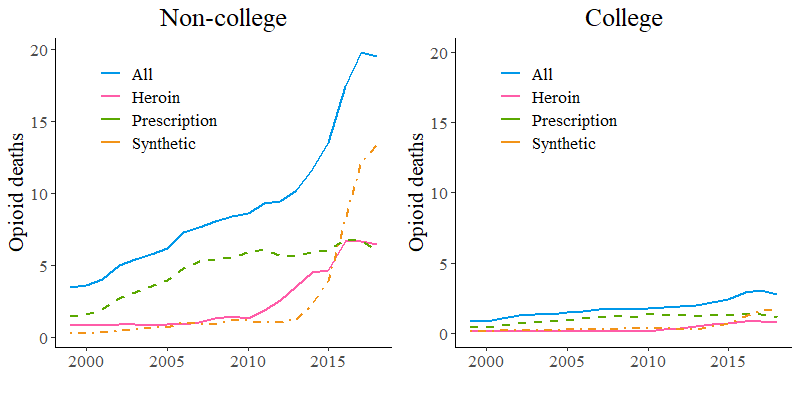
\includegraphics[scale=0.5]{ODD.png}
    \end{center}

    {\footnotesize \textit{Opioid deaths for both the non-college and college-educated as measured per 100,000 people in the respective education class (\textcolor{fgre}{Greenwood, Guner and Kopecky, 2022})}}
    
\end{frame}

\begin{frame}

    \label{main_idea}
    \frametitle{Main idea} % Title
    \framesubtitle{}  % Subtitle
    \rmfamily % Font
    
    \begin{wideitemize}
        \item Opioid misuse can lead the victims to negative Labor Market Outcomes (\textcolor{fblu}{LMOs})
        \item The impact of substance abuse on LMOs might be mediated by labor market regulations
        \item \textcolor{fblu}{Minimum wage rates} can affect this impact 
        \vspace{9pt}
        \begin{wideitemize}
            \item[\textcolor{fblu}{\textbullet}] Negatively, through their effect on \textcolor{fblu}{labor demand for low-skill jobs} 
            \item[\textcolor{fblu}{\textbullet}] Positively, if they address the reasons that cause \textcolor{fblu}{addiction} in the first place \(\to\) \textcolor{fblu}{Deaths of despair}
        \end{wideitemize}
        %\item The dominance of each effect depends on how \textcolor{fblu}{binding} minimum wage rates are across labor markets
        \item How \textcolor{fblu}{binding} minimum wage rates are across labor markets is the relevant measure
    \end{wideitemize}

    \hyperlink{min_wage_plot}{\beamerbutton{Minimum wage trends}}
    \hyperlink{min_wage_plot_allstates}{\beamerbutton{All states}}

\end{frame}

\begin{frame}

    \frametitle{In this paper I ask} % Title
    \framesubtitle{}  % Subtitle
    \rmfamily % Font
    
    \begin{wideitemize}
        \item Do the effects of \textcolor{fblu}{Opioid Use Disorders} (\textcolor{fblu}{OUDs}) on labor market outcomes vary depending on minimum wage bindingness?
        %\item If so, how have these policies shaped the ongoing Crisis?
        %\item Is the interaction homogeneous across States, or can we expect differences across labor markets?
    \end{wideitemize}

    \vspace{9pt}
    I will use \textcolor{fblu}{changes in state prescription drug regulations} as a source of variation
    \vspace{9pt} 
    
    \begin{wideitemize}
        \item These changes can be seen as \textcolor{fblu}{exogeneous} from the \textcolor{fblu}{county level}
    \end{wideitemize}
    
\end{frame}


\begin{frame}

    \frametitle{Prescription policies} % Title
    \framesubtitle{}  % Subtitle
    \rmfamily % Font
    
    \begin{wideitemize}
        \item More stringent regulations on opioid access can make the victims to 
        \vspace{9pt}
        \begin{wideitemize}
            \item[\textcolor{fblu}{\textbullet}] \textcolor{fblu}{Quit}, which might imply some disutility, or
            \item[\textcolor{fblu}{\textbullet}] \textcolor{fblu}{Switch to the black market}
        \end{wideitemize}
        \item This decision affects the MPL of the worker
        \item In this scenario, minimum wage rates might
        \vspace{9pt}
        %\begin{wideitemize}
        %    \item[\textcolor{fblu}{\textbullet}] Improve labor outcomes if better living conditions tackle the causes of addiction and relapsing (\(\textcolor{fblu}{w_{min}}\) \textcolor{fblu}{not binding})
        %    \item[\textcolor{fblu}{\textbullet}] Foster addiction, if quitting doesn't improve labor prospects because \(\textcolor{fblu}{w_{min}}\) \textcolor{fblu}{binding} 
        %\end{wideitemize}
        \begin{wideitemize}
            \item[\textcolor{fblu}{\textbullet}] Increase the rates of unemployment of the workers that don't quit (\(\textcolor{fblu}{w_{min}}\) \textcolor{fblu}{binding})
            \item[\textcolor{fblu}{\textbullet}] Not have an impact on employment rates for addicted workers (\(\textcolor{fblu}{w_{min}}\) \textcolor{fblu}{not binding})
        \end{wideitemize}
    \end{wideitemize}
    
\end{frame}

\begin{comment}
\begin{frame}

    \frametitle{Prescription policies} % Title
    \framesubtitle{}  % Subtitle
    \rmfamily % Font

    \begin{equation*}
        \begin{aligned}
            w^{min}\,\,\text{not binding} & \xrightarrow[\text{passed}]{\text{Prescription law}}
            \begin{cases}
                \text{\textcolor{fblu}{Quit}} \\
                \text{LMOs improve} \\
                \downarrow \text{Prescription rates} \\
                \downarrow \text{Mortality} \\
            \end{cases} \\
            & \\
            w^{min}\,\,\text{binding} & \xrightarrow[\text{passed}]{\text{Prescription law}}
            \begin{cases}
                \text{\textcolor{fblu}{Black market}} \\
                \text{LMOs worsen} \\
                \downarrow \text{Prescription rates} \\
                \uparrow \text{Mortality} \\
            \end{cases} \\ 
        \end{aligned}
    \end{equation*}

\end{frame}
\end{comment}

\begin{frame}

    \frametitle{Prescription policies} % Title
    \framesubtitle{}  % Subtitle
    \rmfamily % Font

    \begin{wideitemize}
        \item Minimum wage bindingness can affect the decision of the worker to quit opioids
        \item This impact is \textcolor{fblu}{ambiguous} and depends on the \textcolor{fblu}{cost of quitting} and the \textcolor{fblu}{impact of addiction on productivity}
        \item Unless minimum wages force the worker to quit strongly enough, we should see a \textcolor{fblu}{negative impact on employment rates} where the minimum wage is \textcolor{fblu}{more binding}
    \end{wideitemize}

\end{frame}

\begin{frame}

    \frametitle{Contribution} % Title
    \framesubtitle{}  % Subtitle
    \rmfamily % Font

    \begin{wideitemize}
        \item \textcolor{fgre}{Cengiz et al. (2019)} \(\to\) minimum wage changes reduced employment in low-wage jobs of tradeable sectors
        \item \textcolor{fgre}{Aliprantis, Fee, and Schweitzer (2023)} \(\to\) large and significant negative impact of prescription rates on labor force participation
        \item \textcolor{fgre}{Alpert, Powell, and Pacula (2018)} \(\to\) positive relation between OxyContin misuse and heroin deaths 
    \end{wideitemize}

    \vspace{9pt}
    \textbf{Contribution}: shedding light on how the labor effects of the \textcolor{fblu}{Opioid Crisis} have been affected by \textcolor{fblu}{minimum wage rates}
    \vspace{9pt}
    
    \begin{wideitemize}
        \item Interest in how \textcolor{fblu}{labor market regulations} interact with \textcolor{fblu}{Substance Abuse Disorders}
    \end{wideitemize}
    
\end{frame}

